% ============================================================
% 1B: Tiling
% ============================================================

\subsection{Task 1B: Tiling}

\subsubsection{Baseline Profiling}
The L1 Data (L1-D) cache size on the tested system is 448 KiB. Profiling the baseline (naive) 2D convolution yields an L1-D MPKI of 0.06 for a 2048x2048 matrix with a kernel size of 5.

\subsubsection{Implementation}
The tiled 2D convolution is implemented by dividing the output matrix into square blocks of a fixed dimension, \texttt{sz}[cite: 5]. The outer loops iterate over the tile origins (\texttt{oyT} and \texttt{oxT}) to process the image block by block[cite: 5]. Within each tile block, the output values are initialized to zero, and the kernel loops (\texttt{ky} and \texttt{kx}) accumulate the weighted inputs strictly within the local spatial bounds[cite: 5]. This reorders the memory accesses to keep the active working set confined within the cache.

\begin{figure}[H]
    \centering
    \begin{subfigure}{0.48\textwidth}
        \centering
        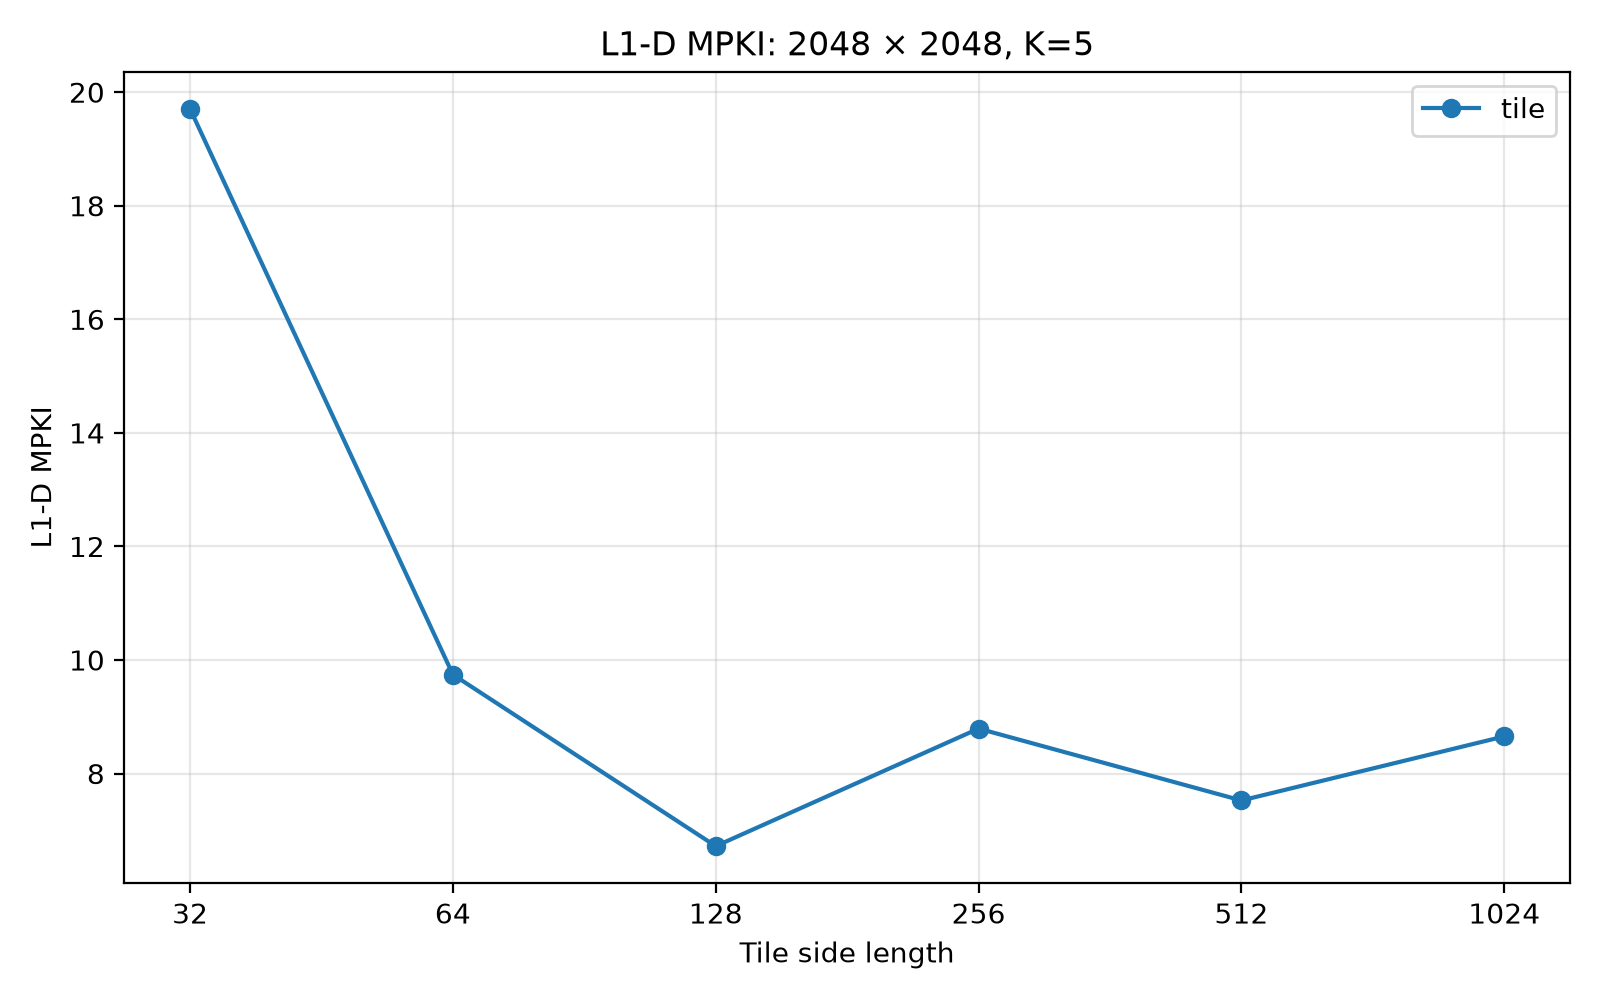
\includegraphics[width=\linewidth]{plots/task1b/plots_1d/n2048_l1_mpki_k5.png}
        \caption{L1-D MPKI vs. Tile Size (2048x2048)}
        \label{fig:tiling_mpki_1d}
    \end{subfigure}
    \hfill
    \begin{subfigure}{0.48\textwidth}
        \centering
        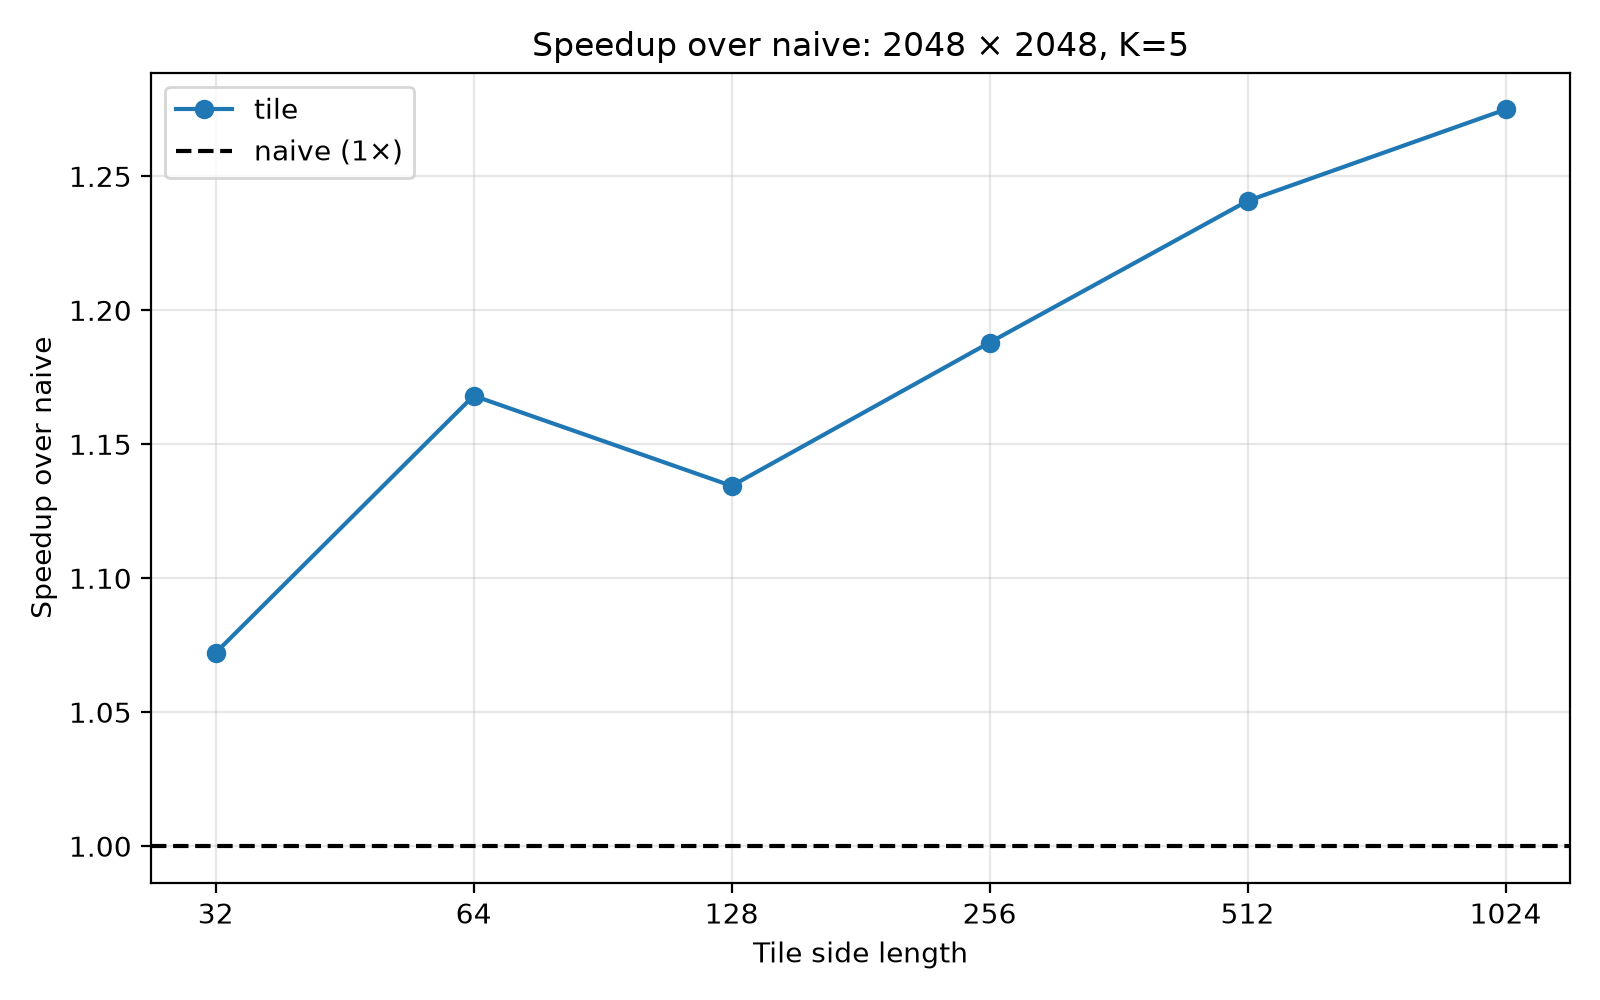
\includegraphics[width=\linewidth]{plots/task1b/plots_1d/n2048_speedup_k5.png}
        \caption{Speedup vs. Tile Size (2048x2048)}
        \label{fig:tiling_speedup_1d}
    \end{subfigure}
    \caption{Cache behavior and performance for a 2048x2048 matrix at $K=5$.}
    \label{fig:task1b_1d}
\end{figure}

\begin{figure}[H]
    \centering
    \begin{subfigure}{0.48\textwidth}
        \centering
        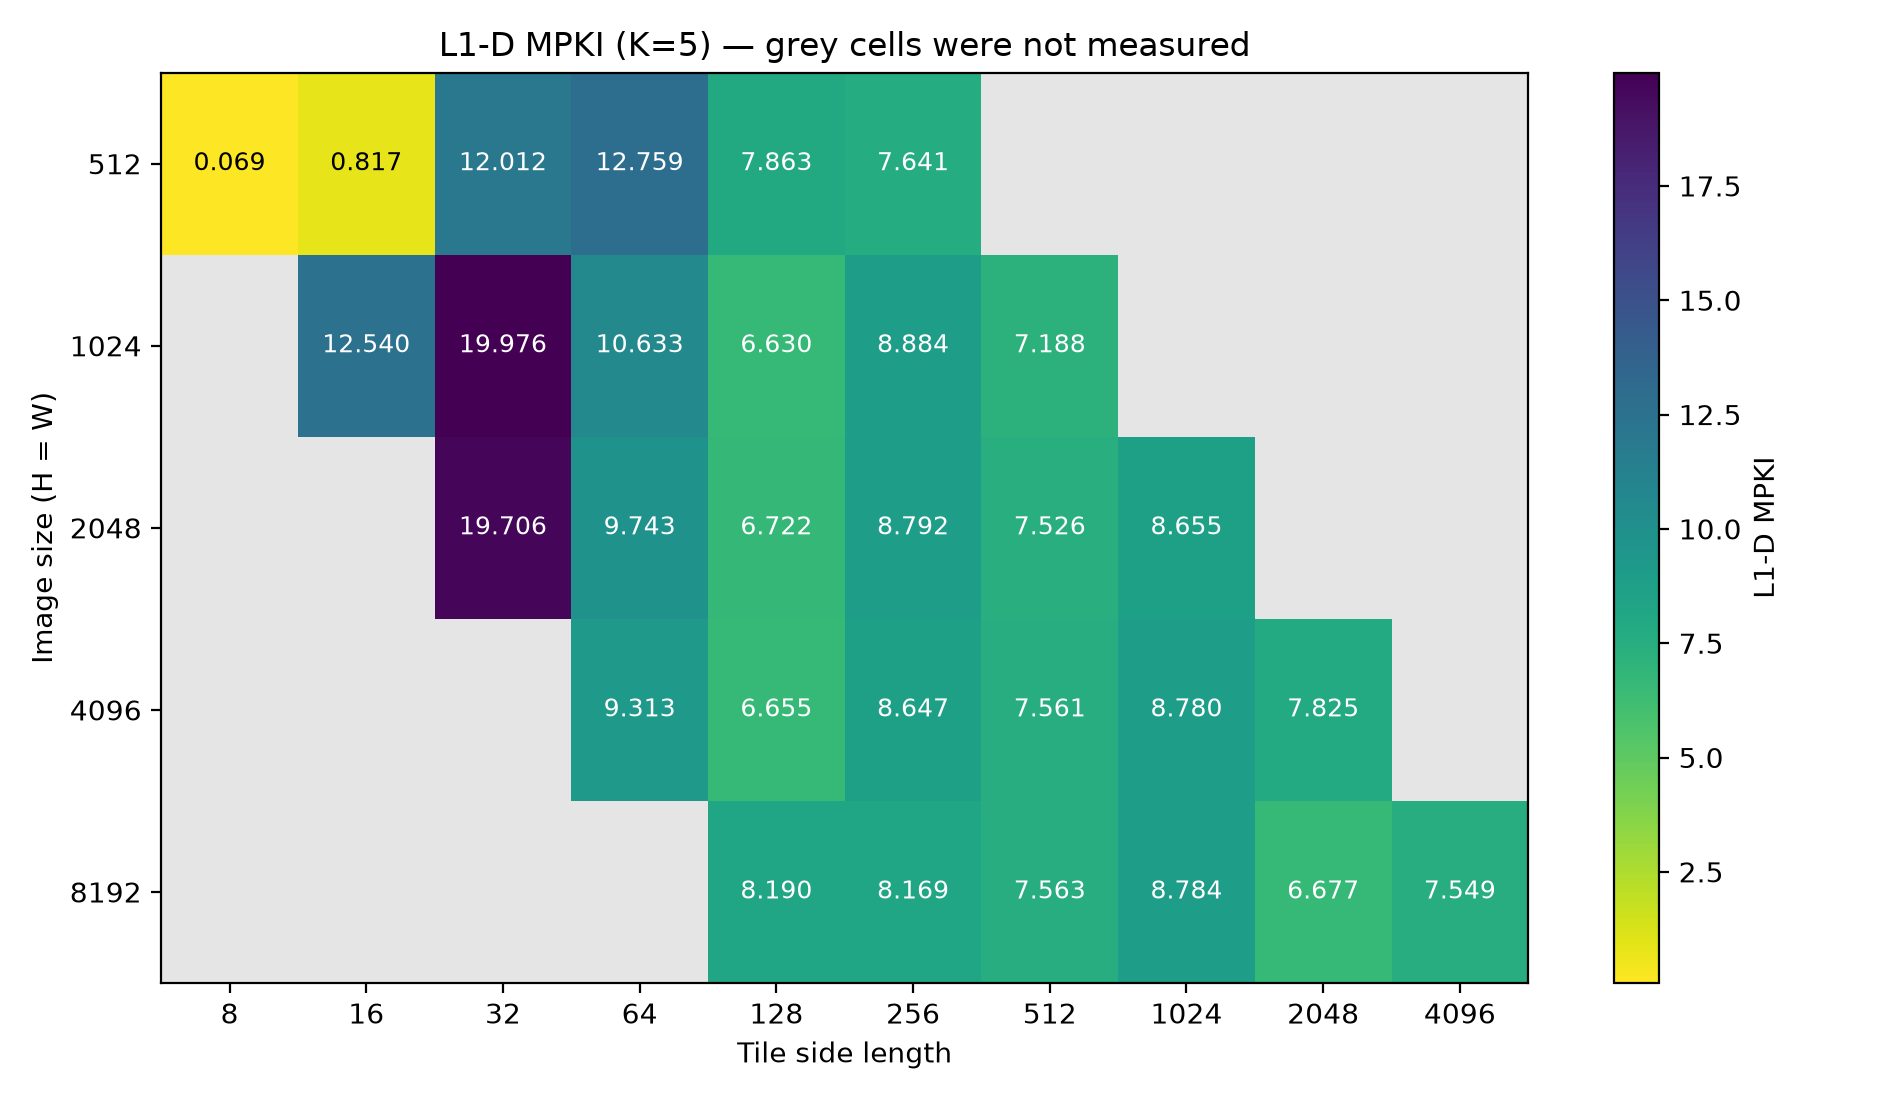
\includegraphics[width=\linewidth]{plots/task1b/plots_2d/l1_mpki_heatmap_k5.png}
        \caption{L1-D MPKI Heatmap}
        \label{fig:tiling_mpki_heatmap}
    \end{subfigure}
    \hfill
    \begin{subfigure}{0.48\textwidth}
        \centering
        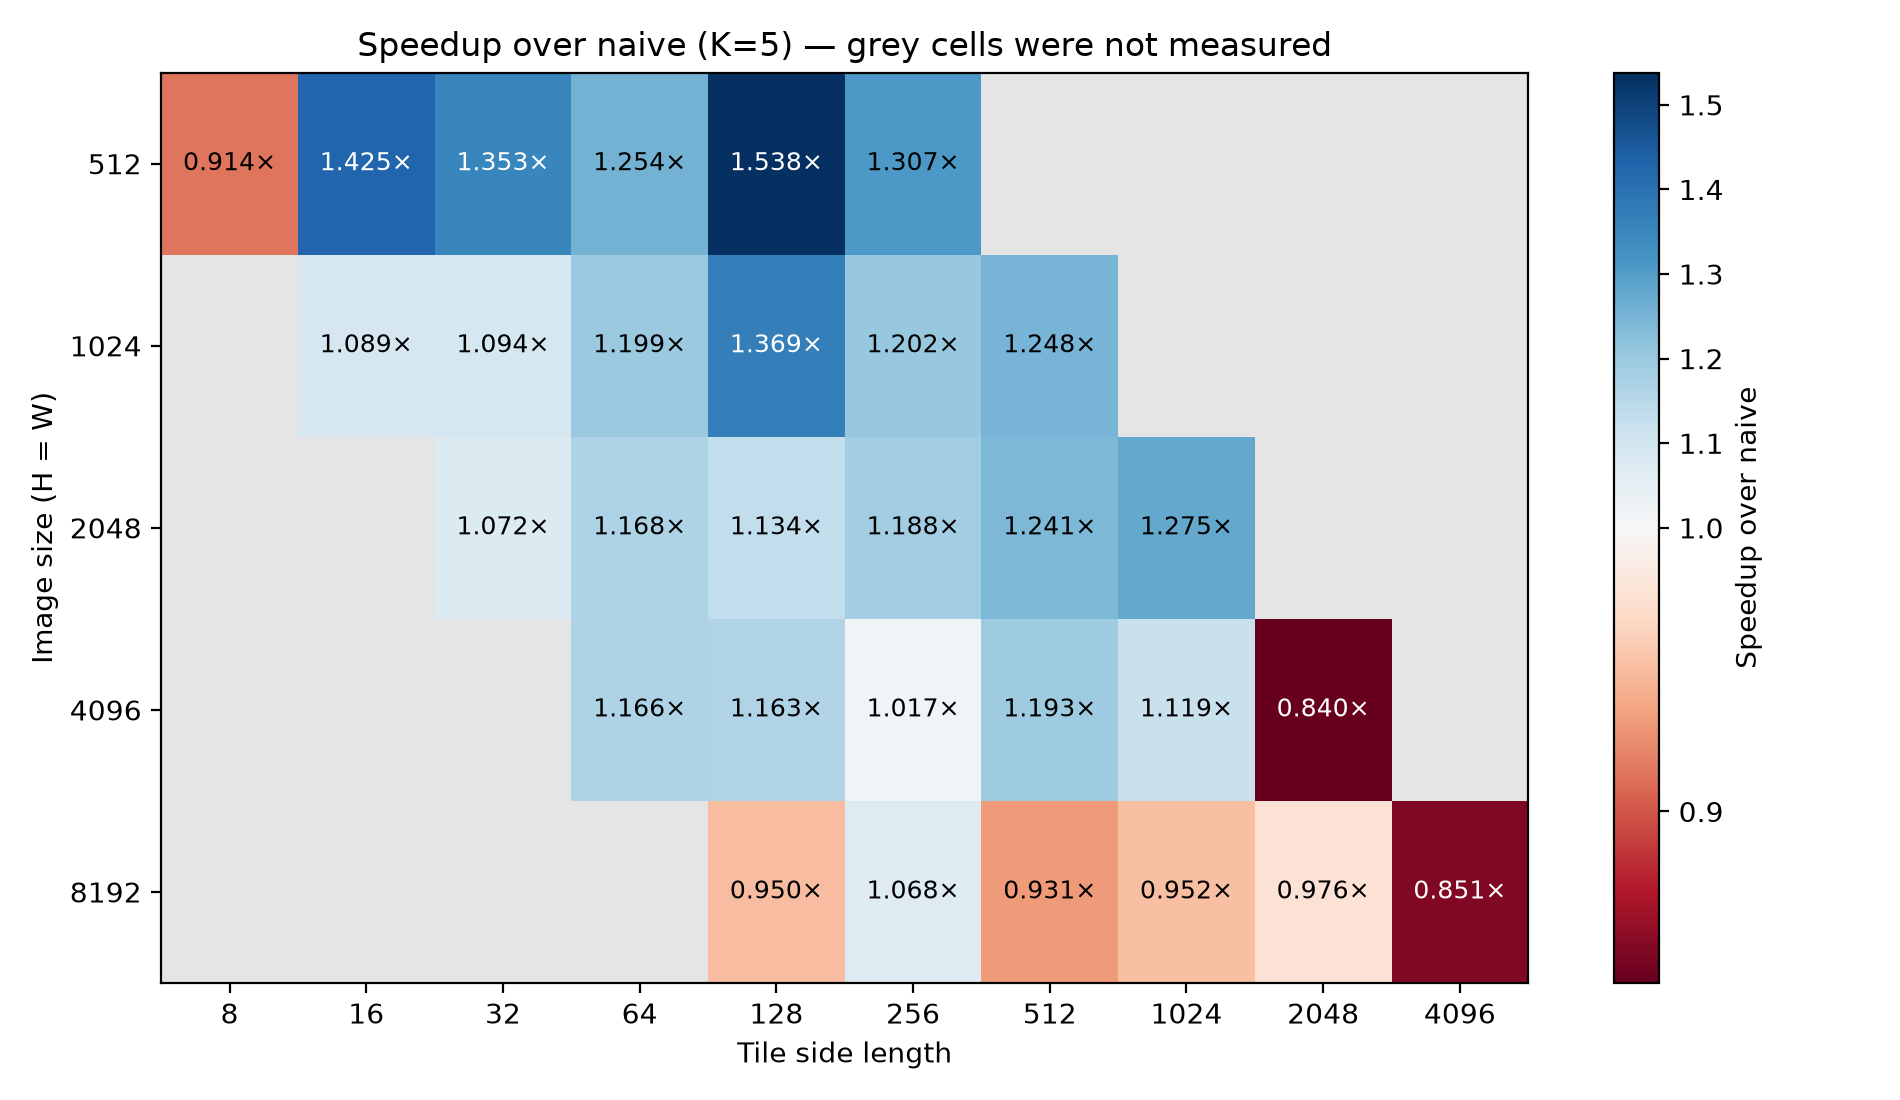
\includegraphics[width=\linewidth]{plots/task1b/plots_2d/speedup_heatmap_k5.png}
        \caption{Speedup Heatmap}
        \label{fig:tiling_speedup_heatmap}
    \end{subfigure}
    \caption{Performance trends across varying matrix sizes and tile sizes ($K=5$).}
    \label{fig:task1b_2d}
\end{figure}

\subsubsection{Analysis}

\begin{enumerate}
    \item \textbf{Report the changes in L1-D MPKI observed when moving from naive to tiled 2D convolution. Justify your observations.} \\
    The L1-D MPKI increased significantly, jumping from just 0.06 in the naive version to a range of $\sim$6 to 19 in the tiled version. The naive implementation accesses memory in long, predictable linear streams, which hardware prefetchers can easily identify and hide. Tiling breaks these accesses into short, discontinuous blocks, which disrupts the hardware prefetchers and exposes the actual cache miss rate.
    
    \item \textbf{How did L1-D MPKI vary across different matrix sizes and tile sizes? Explain your findings in terms of the cache hierarchy and working set sizes.} \\
    MPKI hits a minimum at intermediate "sweet spot" tile sizes (e.g., 128 for a 2048x2048 matrix). If the tile size is too large (e.g., $\ge$ 512), the working set memory footprint exceeds the system's 448 KiB L1 cache capacity, resulting in capacity misses. If the tile size is too small (e.g., 32), the boundary overhead and frequent pointer jumps increase the relative miss rate without providing additional cache benefits.
    
    \item \textbf{Did you achieve a speedup? If yes, quantify the improvement and identify the contributing factors. If not, analyze the limiting factors and propose possible solutions.} \\
    Yes, a speedup was achieved. For a 2048x2048 matrix, the speedup reached $\sim$1.27$\times$ at a tile size of 1024, and peaked at 1.53$\times$ for a 512x512 matrix with a tile size of 256. Despite the higher L1-D MPKI caused by prefetcher disruption, overall execution time improved because tiling maximizes data reuse in the larger L2 and Last Level Caches (LLC), significantly reducing the high latency penalty of fetching data from main memory.
\end{enumerate}